\chapter{First Chapter}
\label{sec:chapter_1}

This is the first chapter. You may add nomenclatures as shown here, following the DRY principle.

\nomenclature{DRY}{Don't Repeat yourself}

\section{First Section}
\label{sec:chapter_1-1}

This is the first section. You may cite papers as such~\cite{Newton:1687eqk}. You may also refer to tables in the thesis as \cref{tab:placeholder_data}


\begin{table}
	\centering
	\caption{Comparison of experimental results across different model architectures using placeholder data.}
	\label{tab:placeholder_data}
	\begin{tabular}{lcccc}
		\toprule
		\textbf{Method}   & \textbf{Precision} & \textbf{Recall} & \textbf{F1-Score} & \textbf{Latency (ms)} \\
		\midrule
		Baseline Model    & 0.82               & 0.79            & 0.80              & 12.4                  \\
		Variant A         & 0.85               & 0.81            & 0.83              & 15.1                  \\
		Variant B         & 0.89               & 0.84            & 0.86              & 18.7                  \\
		\textbf{Proposed} & \textbf{0.94}      & \textbf{0.91}   & \textbf{0.92}     & \textbf{22.3}         \\
		\bottomrule
	\end{tabular}
\end{table}


\section{Second Section}
\label{sec:chapter_1-2}

This is another section. Here we refer to the equation
\begin{equation}
	E = mc^2 ,
	\label{eq:my-formula}
\end{equation}
where we can also define the symbols in \cref{eq:my-formula} in the nomenclature as shown below (in the code).

\nomenclature{$E$}{Energy}
\nomenclature{$m$}{Mass}
\nomenclature{$c$}{Speed of light}

\chapter{Second Chapter}
\label{sec:chapter_2}

This is another chapter. You may reference an earlier section, \textit{e.g.}, ``as mentioned in \cref{sec:chapter_1} and \cref{sec:chapter_1-2}, ...''. You may also refer to figures in the thesis as \cref{fig:placeholder}.

\begin{figure}
	\begin{center}
		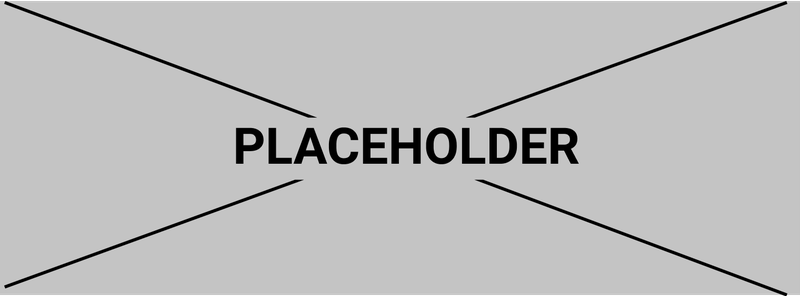
\includegraphics[width=0.95\textwidth]{figures/placeholder.png}
	\end{center}
	\caption{\textbf{A placeholder image.}\ This image shows a placeholder}\label{fig:placeholder}
\end{figure}

